
\chapter{Introduction}

\section{Motivation}


\section{Distant Speech Recording (DSR)}
Figure~\ref{fig:DSR_scenario} shows the setup of DSR used in this work. This work considers a single speech source placed distant ($400$~cm to few meters) from the microphone. Noise is assumed to be additive with reverberated speech. The source and receiver are assumed to be stationary. The speech is recorded using a single microphone. Microphone output in such a scenario is a degraded version of the original speech. The effects of reverberation and noise are predominant in such a case. Such degradation will not happen for the close-talking case since the microphone is placed very close to the source. The speech quality and automatic speech recognition (ASR) performance of DSR is poor because of such degradation. Hence, there is a need for improving the same. 
\iffalse
\begin{itemize}
\item Why use DSR ?
\item Difference between close-talking and DSR
\item Effect on speech quality and ASR in DSR
\end{itemize}
\fi
\begin{figure}
\centering
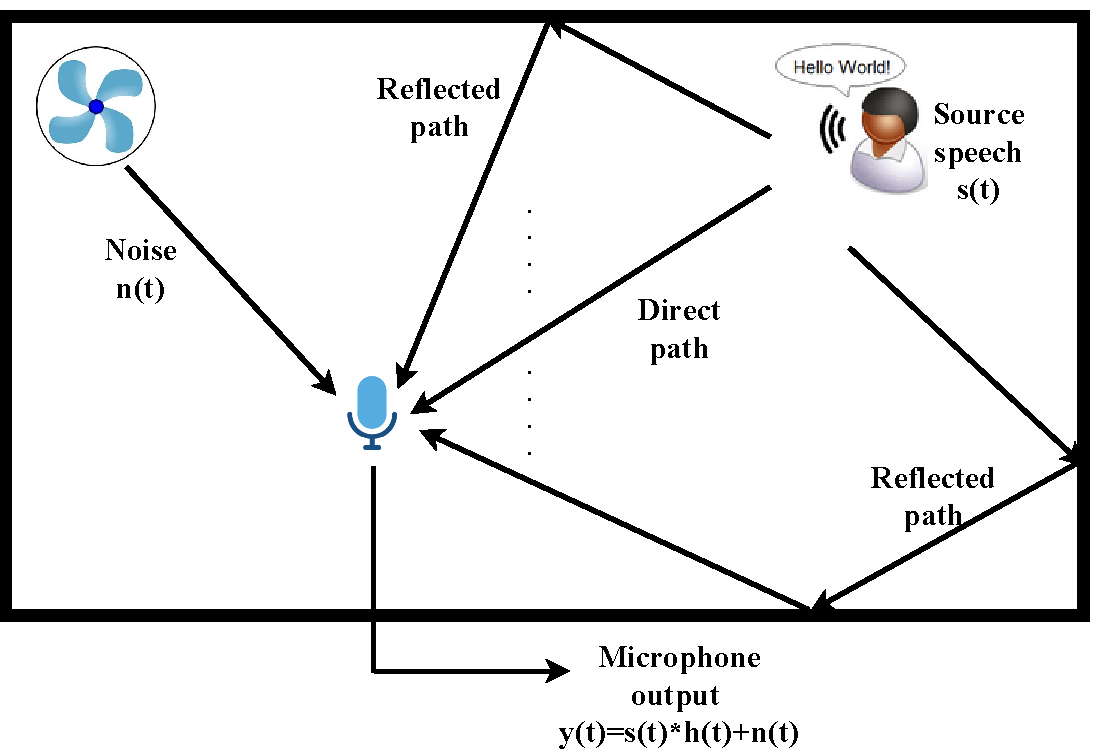
\includegraphics[width=\linewidth]{DSR_scenario.pdf}
\caption{DSR scenario}
\label{fig:DSR_scenario}
\end{figure}

\section{Reverberation}
Speech originating from a source placed distant from the receiving microphone undergoes multiple reflections. The microphone output will be the superposition of original source along with these delayed and attenuated versions of the original source. This effect is known as reverberation. The reverberated speech $y_R(n)$ can be represented as convolution of clean speech $s(n)$ and room impulse response (RIR) $h(n)$. Mathematically,
\begin{equation}
y_R(n)=h(n)*s(n) = \sum_{l=0}^{L-1}h(l)s(n-l),
\end{equation}
where $L$ represents the number of taps used to represent $h(n)$. Reverberated speech is assumed to be additive with noise. Mathematically, degraded speech $y(n)$ due to the effects of reverberation and noise can be represented as,
\begin{equation}
y(n)=y_R(n)+z(n)=h(n)*s(n)+z(n),
\end{equation}
where, $z(n)$ represents the noise. The effects of reverberation is different from the effects of echo.

The effects of reverberation depends on the properties of clean speech as well as RIR. Since reverberation dependent on the original source (clean speech), compensating for the effects of reverberation and blindly estimate the clean speech will be challenging.  

Speech originating from a source undergoes multiple reflections in a closed room. When this speech is captured using a microphone distant from the source (typically 30 cm to few meters), the microphone output is a superposition of the speech along with the delayed and attenuated copies of the signal referred to as reverberated speech~\cite{naylor2010speech}. Additionally, the microphone will capture background noise originating from other sources. The resulting microphone output in such a distant speech recording (DSR) setting is a degraded version of the original speech signal. The presence of such degradations impedes speech intelligibility~\cite{kinoshita2016summary}  and automatic speech recognition (ASR)~\cite{barker2018fifth, barker2015third} performance. The amount of degradation depends on the source and microphone positions, characteristics of the room and the noise~\cite{naylor2010speech,kinoshita2016summary}. To improve performance, it is desirable to compensate for these degradations.
\iffalse
\begin{itemize}
\item What is it ?
\item Representation using RIR
\item Differentiate reverberation from echo
\item Why it is challenging ?
\item Combined effect with noise
\end{itemize}
\fi
\section{Objective of the thesis}
\begin{itemize}
\item Improve speech quality of a single-channel DSR recording
\item Compensation for reverberation and noise
\item Improve ASR
\end{itemize}

\section{Contributions}
The main contribution of this work is incorporating various properties of the RIR spectrogram in a NMF based framework for dereverberation and denoising. Three different approaches to incorporate different properties of the RIR spectrogram are discussed in this work. Firstly, the cost function for NMF based dereverberation method is modified to introduce three different RIR structures - sparsity, frequency envelope and early part of the RIR spectrogram. The second part of the work proposes a NMF based speech enhancement method based on separability approximation on the RIR spectrogram. The model helps in separating the temporal and frequency effects of reverberation on clean speech and improving the speech enhancement results. The third work utilizes the low-rank nature of the RIR spectrogram to represent the joint effect of reverberation and noise using a NMF model. Further, an algorithm based on this model is shown to improve speech enhancement and ASR results when compared with other NMF based approaches in the literature.

\iffalse
\begin{itemize}
\item incorporate various constraints on RIR spectrogram in a NMF based dereverberation framework
\begin{itemize}
\item model sparsity, frequency envelope, early part of RIR
\item incorporate the constraints in cost function
\end{itemize}
\item A novel NMF based method to handle reverberation and noise jointly
\begin{itemize}
\item propose NMF models for RIR spectrogram (separability assumption, low-rank model)
\item incorporate these models along with NMF models for clean speech and noise spectrograms
\item better constrained model resulting in proper RIR and clean speech estimates
\item improvement in enhancement and ASR results
\item better understanding of effects of reverberation on clean speech bases and activations
\end{itemize}
\end{itemize}
\fi
\section{Organization of thesis}
Figure~\ref{fig:Thesis_chapters} shows the organization of rest of the thesis. Chapter~\ref{chapter:lit} reviews various speech dereverberation and denoising methods in literature. Chapter~\ref{chapter:rir} describe some of the time and frequency domain structure of RIR. These structure are utilized in this work. Chapter~\ref{chapter:icassp2017} discusses NMF based dereverberation methods that incorporates various meaningful constraints on RIR spectrogram. Chapter~\ref{chapter:interspeech2018} discusses a speech enhancement method based on separability assumption of the RIR spectrogram. Chapter~\ref{chapter:trans2020} discusses the speech enhancement method based on low-rank approximation of the RIR spectrogram. In Chapter~\ref{chapter:conclusion}, the work is concluded with discussions and possible future directions in incorporating these methods for other applications.
\begin{figure}
\centering
\includegraphics[width=\linewidth]{Thesis_chapters.pdf}
\caption{Thesis chapters}
\label{fig:Thesis_chapters}
\end{figure}
